\documentclass{sigchi}

% Remove or comment out these two lines for final version
\toappearbox{\Large Submitted to CSCW'13. \\Do not cite, do not circulate.}
\pagenumbering{arabic}% Arabic page numbers for submission. 

% Use \toappear{...} to override the default ACM copyright statement (e.g. for preprints).

% Load basic packages
\usepackage{balance}  % to better equalize the last page
\usepackage{graphics} % for EPS, load graphicx instead
\usepackage{times}    % comment if you want LaTeX's default font
\usepackage{url}      % llt: nicely formatted URLs
\usepackage{listings}
\usepackage{gensymb}
\usepackage{multirow}
\usepackage{color}

%\usepackage{caption}
%\usepackage{subcaption}

% llt: Define a global style for URLs, rather that the default one
\makeatletter
\def\url@leostyle{%
  \@ifundefined{selectfont}{\def\UrlFont{\sf}}{\def\UrlFont{\small\bf\ttfamily}}}
\makeatother
\urlstyle{leo}


% To make various LaTeX processors do the right thing with page size.
\def\pprw{8.5in}
\def\pprh{11in}
\special{papersize=\pprw,\pprh}
\setlength{\paperwidth}{\pprw}
\setlength{\paperheight}{\pprh}
\setlength{\pdfpagewidth}{\pprw}
\setlength{\pdfpageheight}{\pprh}


% create a shortcut to typeset table headings
\newcommand\tabhead[1]{\small\textbf{#1}}


%************* Andreas Additions
%% Usage: You do not need \begin{enumerate} and \end{enumerate} statements.
%% Just the \squishlist and \squishend statements, and the \items's in between.
%% If you do not want a bulleted list, you can add " [(a)]" after the fist \item,
%% " [(b)]" after the second one, etc, to get a, b, ... bullets...
%% (or 1, 2, 3... can replace the a, b, c...)

\newcommand{\squishlist}{
 \begin{list}{$\bullet$}
 {
  \setlength{\itemsep}{0pt}
  \setlength{\parsep}{0pt}   %3pt
  \setlength{\topsep}{0pt}   %3pt
  \setlength{\partopsep}{0pt}
  \setlength{\leftmargin}{1.5em}
  \setlength{\labelwidth}{1em}
  \setlength{\labelsep}{0.5em} } }

\newcommand{\squishend}{
  \end{list}  }

% Alter some LaTeX defaults for better treatment of figures:
    % See p.105 of "TeX Unbound" for suggested values.
    % See pp. 199-200 of Lamport's "LaTeX" book for details.
    %   General parameterbnos, for ALL pages:
    \renewcommand{\topfraction}{0.9}	% max fraction of floats at top
    \renewcommand{\bottomfraction}{0.8}	% max fraction of floats at bottom
    %   Parameters for TEXT pages (not float pages):
    \setcounter{topnumber}{2}
    \setcounter{bottomnumber}{2}
    \setcounter{totalnumber}{4}     % 2 may work better
    \setcounter{dbltopnumber}{2}    % for 2-column pages
    \renewcommand{\dbltopfraction}{0.9}	% fit big float above 2-col. text
    \renewcommand{\textfraction}{0.07}	% allow minimal text w. figs
    %   Parameters for FLOAT pages (not text pages):
    \renewcommand{\floatpagefraction}{0.7}	% require fuller float pages
	% N.B.: floatpagefraction MUST be less than topfraction !!
    \renewcommand{\dblfloatpagefraction}{0.7}	% require fuller float pages

	% remember to use [htp] or [htpb] for placement


% Adds a space between the text and the [T]op \hline
% Must use the \T *within* a cell, not right after the \hline
\newcommand\T{\rule{0pt}{2.5ex}}%{3.1ex}}

% Adds a space between the text and the [B]ottom \hline
% Must use the \B *within* a cell, not right after the \hline
\newcommand\B{\rule[-1ex]{0pt}{0pt}}%[-1.7ex]{0pt}{0pt}}

% Enable grayed-out text environments, like {\graytext foo}:
\definecolor{gray}{RGB}{163,163,163}
\newenvironment{graytext}{\color{gray}}{\ignorespacesafterend}

%\setlength{\belowcaptionskip}{-3pt}

%************* End Andreas Additions


% Make sure hyperref comes last of your loaded packages, 
% to give it a fighting chance of not being over-written, 
% since its job is to redefine many LaTeX commands.
\usepackage[pdftex]{hyperref}
\hypersetup{
pdftitle={SIGCHI Conference Proceedings Format},
pdfauthor={LaTeX},
pdfkeywords={SIGCHI, proceedings, archival format},
bookmarksnumbered,
pdfstartview={FitH},
colorlinks,
citecolor=black,
filecolor=black,
linkcolor=black,
urlcolor=black,
breaklinks=true,
}


% End of preamble. Here it comes the document.
\begin{document}

\title{EchoTree: Engaged Conversation when Capabilities are Limited}

% Note that submissions are blind, so author information should be omitted


%\numberofauthors{2}
%\author{
%  \alignauthor Andreas Paepcke\\
%    \affaddr{Stanford University}\\
%    \affaddr{Stanford, CA}\\
%    \email{paepcke@cs.stanford.edu}
%  \alignauthor Caroline Pantofaru, Dirk Thomas, Austin Hendrix, Sarah Elliot, Sharon Marzouk\\
%    \affaddr{Willow Garage}\\
%    \affaddr{Menlo Park, CA}\\
%    \email{\{pantofaru,dthomas,ahendrix,selliott,smarzouk\}@willowgarage.com}
%    }

% \author{
%  \parbox[t]{18.0cm}{\centering 
%    {\em Andreas Paepcke\**}, 
%    {\em Caroline Pantofaru\**\**}, 
%    {\em Dirk Thomas\**\**}, 
%    {\em Austin Hendrix\**\**}, 
%    {\em Sharon Marzouk\**\**},
%    {\em Sarah Elliot\**\**}}\\
%  \\
%  \parbox[t]{5.0cm}{\centering
%         \**Stanford University\\
%         353 Serra Mall\\
%         Stanford, CA 94305\\
% 	paepcke@cs.stanford.edu}\\
%  \\
%  \parbox[t]{10.0cm}{\centering
%     	\**\**Willow Garage\\
% 	68 Willow Road\\
% 	Menlo Park, CA 94025\\
%        \{pantofaru,dthomas,ahendrix,smarzouk,selliott@willowgarage.com\}}
% }

% Teaser figure can go here
%\teaser{
%  \centering
%  \includegraphics{Figure1}
%  \caption{Teaser Image}
%  \label{fig:teaser}
%}

\maketitle

\begin{abstract}
We describe the collaborative use of word tree visualizations, {\em
  EchoTree}s, to facilitate face-to-face, and remote communication
with speech and movement impaired individuals. EchoTree is designed to
bridge the inevitable conversational dead space while the impaired
person uses assistive technologies to generate written, or
artificially spoken sentences. Visualizations that guess multiple
conversational directions in which the impaired person might be headed
keep conversation partners engaged. Partners may call out
possibilities, which the impaired person can confirm or
dismiss. Correct guesses accelerate conversational progress. EchoTrees
are browser based and interactive. Multiple parties may view, and
interact with the same stream of EchoTrees from desktops, tablets, or
smartphones. The application may also be used for collaborative,
geographically remote story telling games, whose participants may, or
may not be pysically impaired. We describe our implementation, and
provide preliminary measurements of how effectively EchoTrees predict
conversation flow for one particular underlying set of text
materials. 
  \end{abstract}

\keywords{assistive technology; prolonged engagement; collaborative conversation; story telling, game}

\category{H.5.2}{Information Interfaces And Presentation}{User Interfaces - Interaction styles}

\terms{Human Factors; Design}


\tolerance=400

%\newcommand{\degree}{$^\circ$}

\section{Introduction}
We collaborate with a motion and speech impaired individual, Henry,
who enjoys conversing. Henry's speech impairment is
complete. Quadriplegia, while severely limiting, does allow Henry to
move his head in affirmation or negation. His hand can operate a mouse
button. One of his communication modes is via a text-to-speech system
({\em tts}). A camera mounted on top of his laptop tracks a confetti
sized white dot pasted on the lower left of his glasses. The resulting
cursor control allows Henry to hunt down the keys of an onscreen
keyboard. On a very good day the resulting speed is 15 words per
minute. The tts produces sound once a sentence is complete. Uttering
words as Henry types them would work, but this approach makes it
difficult for listeners to track the very slowly evolving sentences in
their minds. Poor tts performance for some words would additionally
impede comprehension, which is supported by context when a full
sentence is pronounced in a flow.

This slow communication channel results in very frustrating
experiences during gatherings like parties. A guest will make a remark
to Henry, who will go to work on an answer. To the conversation
partner Henry looks frozen, peering at his laptop screen whose back
surface reveals nothing to the expectant partner. Often the potential
conversation partner wanders off bewildered before Henry can finish
his response sentence.

One improvement would be to install a second display on the backside
of Henry's laptop. Inexpensive, USB based options are available. This
option would at least allow a listener to understand that information
is forthcoming. The option does not help as much as possible in
keeping the listener(s) actively involved in the conversation. 

In an attempt to ameliorate the situation further we developed
EchoTree. EchoTree is a distributed, collaborative word
tree. Figure~\ref{fig:echoTree} shows an example.
\begin{figure}
   \centering
   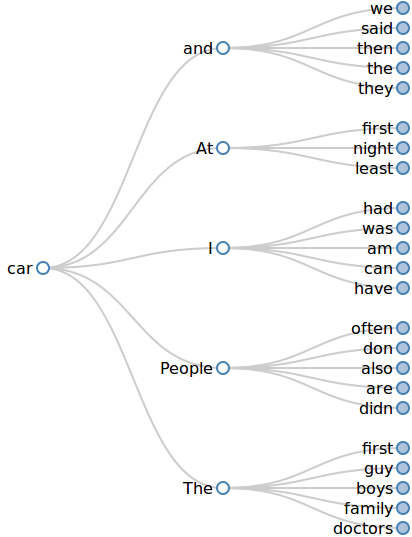
\includegraphics[width=0.6\columnwidth]{Figs/henryBigramsCarTree.png}
   \caption{Screenshot of an EchoTree.}
   \label{fig:echoTree}
\end{figure}
Henry, of course, stands for many individuals with similar
impairments. 
\section{User Experience}
A word tree is read from left to right, beginning with a single word,
the {\em root}. Branching out from the root are words that might
follow the root in an underlying document collection. EchoTree
provides five out branches, which are sorted top to bottom by their
likelihood of being the follower word to the root. Each follower word
candidate itself features five possible followers to the candidate.
The tree thereby presents a number of possible conversation threads
that might begin with the root word.

The underlying collection, of course, impacts the follower
relationship probabilities. We analyze three collections in the
experiment section.

EchoTrees are browser applications that can be viewed anywhere, by
multiple users. In particular, every word that Henry enters on his
laptop induces an EchoTree, which is made available by an EchoTree
server as an interactive Web application. Henry can see the trees as
well. If the word that Henry has in mind to type next is contained in
the tree, Henry can click on the word. The word is transferred to the
{\em sentence box} near the display bottom, which collects his
evolving sentence, and he saves on typing. Once he finishes his next
word, the previous EchoTree is replaced with a new one, rooted at the
latest word. Figure~\ref{fig:todayTree} shows highlighted three words
that were transferred to an input box by clicking on them, one after
the other.
\begin{figure}
   \centering
   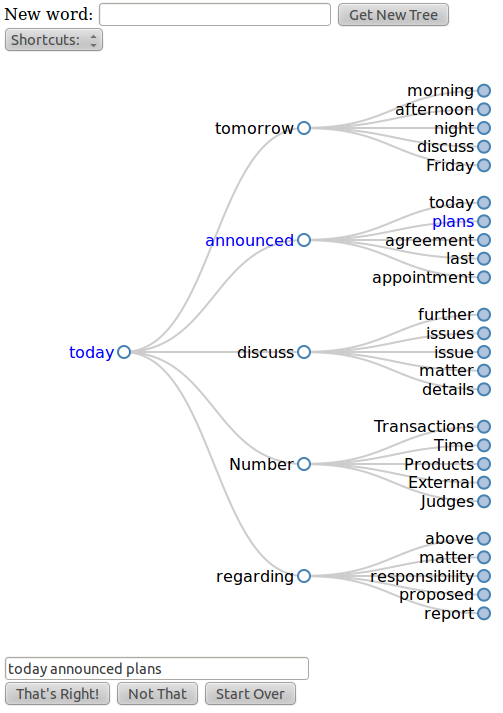
\includegraphics[width=0.6\columnwidth]{Figs/echoTreeRootToday.png}
   \caption{EchoTree re-rooted in `today'. Blue words were user
     selected, adding them to the sentence box.}
   \label{fig:todayTree}
\end{figure}
Beyond providing a word source for Henry to choose from, this
arrangement also enables a number of scenarios where Henry
communicates with conversation partners who have access to his
trees. The important point about each of these scenarios is that
conversation partners remain engaged in the conversation.

For example, the secondary display facing a conversation partner in
the option discussed earlier could always show Henry's current
EchoTree. Alternatively, a conversation partner's smartphone or tablet
can {\em tune in} to Henry's EchoTrees. In either case, informed by the
EchoTree, the partner can guess future words out loud, again saving
Henry some typing and enlivening the conversation. 

Or, the partner can at least spend time exploring EchoTrees on their
own while Henry works: The server allows multiple participants to
generate their own, separate trees, visible only on their own
displays, while still seeing Henry's occasional trees. Henry's trees
are pushed to the client browsers when a new tree becomes available,
because Henry finished a word. The pushed trees replace any tree
currently displayed on the participant's device.

EchoTree delivery to portable devices is thus subscription
based. Participants can in fact subscribe to the EchoTrees of one or
more other participants. The primary scenario for this paper is,
however, to have conversation participants subscribed just to a
disabled person.

Henry or a participant may click or tap on one of the circles in the
tree that currently occupies their display. In response, the tree is
{\em re-rooted}: the selected word becomes the root of a new tree. All
follow words are recomputed, and a new tree is displayed on the
participant's browser, or any other browsers that are subscribed to
trees by the person who generated the new tree.

Alternatively, one may type a new word into the text box at the top,
and click on the button {\em Get New Tree}. This action again creates
a new tree, rooted at the new word, and displayed everywhere.

The EchoTree facility can be used for a number of purposes. In the
context of Henry interacting in a conversation, the facility may be
used as follows. 

\subsection{Collaborative Conversing}
As Henry types words, and corresponding EchoTrees in the browsers of
all tuned in listeners evolve, any word that Henry completes is
additionally appended to the sentence box of all participants'
screens. As listeners actively think ahead, guess where Henry might be
headed, and call out a correct option, Henry can click on the {\em
  That's Right} button, or nod. After the successful guess Henry can
continue, skipping one of more words.

Sometimes participants or Henry may wish to enrich sentences with fill
words. The pull-down menu below the {\em New word} field satisfies
that need (Figure~\ref{fig:shortcuts}). Selecting any of these words
will enter them in the sentence box. Again, in the current
implementation this addition appears in all subscribing views of the
\begin{figure}
   \centering
   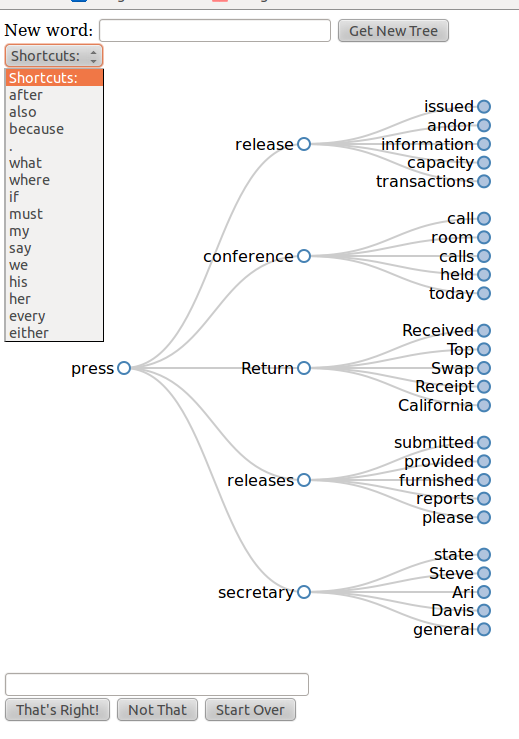
\includegraphics[width=0.4\columnwidth]{Figs/echoTreePulldownSnapshotSmall.png}
   \caption{Shortcut words are available as fillers for the sentence box.}
   \label{fig:shortcuts}
\end{figure}
Note that the use of EchoTrees for collaborative conversation is not
limited to face-to-face situations, like parties. Communication
with Henry via the telephone are also an option. The remote
participant tunes into Henry's EchoTrees, and offers guesses over the
phone. Since Henry nodding assent is not an option in this scenario,
the {\em Not That} button can serve as a negative response.

\subsection{Architecture}

%***** Cover Good-Turing
Figure~\ref{fig:arch} shows how the EchoTree system is
constructed. 
\begin{figure}
   \centering
   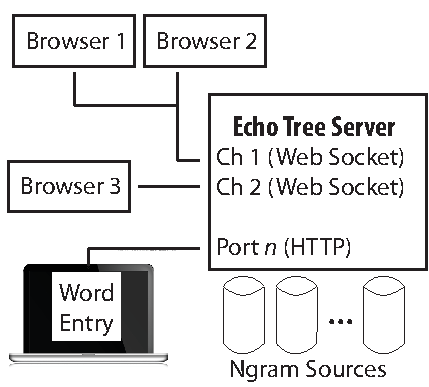
\includegraphics[width=0.5\columnwidth]{Figs/echoTreeArch.pdf}
   \caption{EchoTree architecture. Channels are implemented as
     WebSocket ports. Browsers tune in to different EchoTree channels.}
   \label{fig:arch}
\end{figure}
Central, or distributed EchoTree servers each manage some
number of distinct EchoTree channels. All facilities described above
operated on one channel. All shared EchoTree views are refreshed, and
request re-rooting on one channel. The server computes the trees,
given a root word.

Multiple, unrelated EchoTree sequences may be served by a single
server, using different ports. In Figure~\ref{fig:arch}
Brower~3 is separated from Browsers one and two, which share all
EchoTree transmissions.

Browsers communicate with EchoTree servers via WebSocket connections,
which are bi-directional. This bidirectionality enables the re-rooting
requests from browsers back to the server.

Figure~\ref{fig:arch} also shows an HTTP port family. These ports can
push new words to the echo server, triggering the multicast of a new
EchoTree to all browsers on the respective channel. These HTTP
connections are simpler than the more versatile WebSocket
connections. They are provided for easy connection with word entry
support applications on Henry's machine. For example, Henry uses an
application that offers word completions as he types a word. The HTTP
method of pushing words to the EchoTree server can be attached to this
application. This method allows Henry to focus on typing in his usual
environment, and not being forced to interact with a browser's {\em
  New Word} entry to push a new word (and consequently a new
EchoTree).

Figure~\ref{fig:arch} shows a series of databases with word pair
frequencies that are the basis for the generation of the trees. The
word pairs are word collocation statistics, or {\em bigrams}.  Each
database holds lists of triples: a word, a follower word, and a
frequency count. These bigram counts may originate from any text
collection. Given a root word, EchoTree, like other word tree
visualizations, recursively finds follow-on words, which are chosen by
maximum frequency.

The trees of the above figures are based on bigrams from the Enron
collection ~\cite{enron}. In the following section we examine some
aspects of this underlying collection, which strongly influence the
induced EchoTrees.

\section{Design Considerations}

The cornerstones of EchoTree's design are the choices of underlying
data source, and the language model. But other desicions impact the
user experience as well. In this paper we address the data source
decision. The final word on other design choices is not out yet. But
we next describe the associated considerations.

\subsection{Language Model}
The EchoTree word predictions are based on a model of the English
language. Working with ngrams has served us well. Both bigrams and
trigrams are common choices in Natural Language Processing. Both
options produce plausible word trees, but the display is by necessity
more cluttered when trigrams are shown. Figure~\ref{biTrigrams} shows
a comparison between the two options, using the same root word.
\begin{figure}
   \centering
   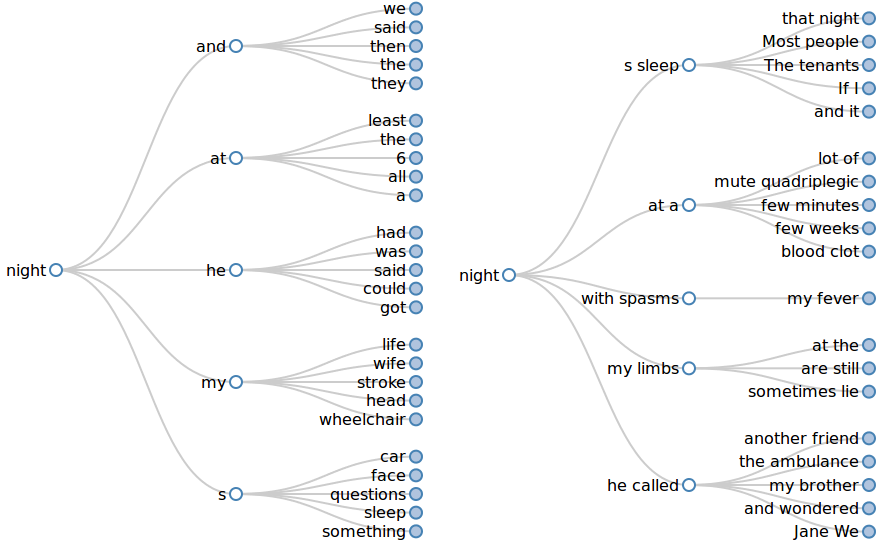
\includegraphics[width=\columnwidth]{Figs/biAndTrigrams.png}
   \caption{Comparing bigram and trigram tree displays.}
   \label{fig:biTrigrams}
\end{figure}
The trigram tree is more expressive, than the bigram tree, but it is
visually denser. Finding words in the trigram display, to then transfer
them to the sentence box is more time consuming than scanning the bigram
version. Depending on word length, the distraction time away from the
onscreen keyboard may outweigh the savings in typing.

The distraction time not only comprises the time it takes to visually
scan the tree, and to move the cursor to a found word via the head
tracker. But the onscreen keyboard must then be re-acquired for
further typing. The tradeoff between typing and retrieving words from the
EchoTree is related to word length: the longer the retrieved word, the
more likely it is that leaving the keyboard is worthwhile.

Word length, in turn, is related to another design choice, the
retention or elimination of stop words.

\subsection{Stopwords}

When designing information retrieval facilities, certain very
frequently occurring words are often disregarded in user queries, and
in underlying index structures. These {\em stopwords} include words
like `the', `that', and `a'. Is stopword elimination appropriate for
our purpose of collaborative conversation? We experimented with both
options, and included examples for both in the the
figures. Figure~\ref{fig:echoTree} was created while retaining
stopwords, while Figure~\ref{fig:todayTree} was constructed with
stopwords removed. 

Clearly, stopword removal tends to display more interesting
words. However, the more complete sentence structure borne from
stopword retention makes it easier for conversation partners to call
out the next word choice, thus saving the disabled typist time. Note
that this time saving is enjoyed in full, because the typist's
attention can continue to dwell on the onscreen keyboard. Short of a
formal study, we have anecdotal evidence from Henry, who prefers to
lay down all words, not leaving out stopwords in spite of the
increased communication expense. A final decision on the stopword
question awaits a study.

\subsection{Data Source}

As described, the probability of any word following another is derived
from word occurrence statistics in an underlying data source. Which
source to use? Intuitively, we suspect might suspect that using a
person's own written materials for the ngram statistics will be
particularly effective in predicting that person's writing. 

One problem with this approach is twofold. For one, a disabled
person's email messages, for example, will tend to be concise. This
brevity in turn limits the amount of material over which ngrams can be
computed. 

A second problem with using personal writing, like email, is that
obtaining the email collection is more difficult now that the material
is stored on company servers, than when email was on everyone's
personal disk. Not many email users would know how to download their
entire email history from their email provider's server. In any event,
such a startup effort is unfortunate for any computer application.

Finally, a third drawback of using personal writings is that EchoTrees
can be quite revealing. The frequency with which a particular word
follows another in one's entire personal corpus should not necessarily
be open to public view.

At the other extreme, we can use a broad source, like Google's
terabyte ngram collection \cite{****}. Its coverage across millions of
Web pages is more or less topic neutral, and thereby maybe universally
applicable. Between these extremes lies the option of utilizing
multiple ngram sets, each from one topic specific collection of Web
pages. Users would choose a configuration that is appropriately close
to their topic of conversation. Maybe the topic specificity would be
beneficial. 

Or, one might argue that neither email, nor Web content, nor ngrams
from scanned books \cite{anc} are optimal for a conversational
context. What if our word choices in conversations is very different
from those of our Web pages?

We conducted an experiment that examined the EchoTree performance of
three datasources, each tested under both bigram and trigram design
variants.

\section{Data Source Performance Experiment}

Our performance measure comprises two components. Both components were
computed automatically.

\subsection{Performance Measures}

We measured both performance components for all six experimental
conditions: three datasources times bigram vs. trigram. The first
performance component is the prediction {\em reliability} with which
EchoTrees predict follow-on words for each successive word in test
sentences. The sentences were taken from collection set-asides over
which no ngrams were collected (see below).

Our automated evaluation pulled one word $W$ after another from each
testing sentence $S$, and constructed an EchoTree with $W$ as its
root. If $W$'s follower appeared in the tree at the tree's first
level, the sentence was assigned one point. If the follower appeared
at the second tree level, one half point was awarded to the
sentence. The reliability measure for $S$ was computed as the sum of
awarded points, normalized to the length of the sentence. The data
source's single reliability performance measure is the average of the
individual sentence performances.

The second performance measure estimates the {\em savings} in
typing. This measure is the percentage of characters that would not
need to be typed in a real life situation, because the respective
words were available in EchoTrees. We counted spaces between words in
the grand sum of letters to be typed. We also counted the click needed to
cause words in the EchoTree to replicate down into the sentence box as
a cost equivalent to typing one character. This method is an
approximation, because of the above mentioned issue of distraction.

\subsection{Tested Data Sources}

The first data source, {\em REC} consists of 10M Web pages we
retrieved from the {\em Recreation} section of the Open Directory
Project (ODP) \cite{****dmoz***}. The project used human input to
categorized Web pages. We eliminated all pages that stemmed from the
ODP site itself, retaining pages from the Recreation target sites one
level deep. We removed all HTML and Javascript from the resulting
pages, then tokenized the remainder using the Stanford NLP Tokenizer
\cite{****Stanford tokenizer}. We then extracted 5,055,284 bigrams,
and 28,423,891 trigrams.

Our second data source is the Fisher collection's transcripts of
11,000 ten-minute telephone conversations {\em FISH}. Each
conversation centers around one topic that was assigned to the paid
conversation dyad participants. We cleaned the collection of embedded
metadata, like the timestamp and source of each speech turn. The
remainder was again tokenized, and we extracted 149,789 bigrams and
93,534 trigrams.

Our third experiment data source, finally is a blog Henry maintains
{\em BLOG}. The snapshot was taken on May 10, 2013, and comprises
1,167 sentences (96.5MB), 12,222 bigrams, and 16,567 trigrams.

In all cases, after removing HTML tags, but before extracting ngrams,
we set aside a portion of each corpus for testing. We used a 10\%
set-aside for REC and FISH, and 5\% for BLOG.

We computed ngram probabilities using the Good-Turing algorithm
\cite{***good-turing***}. This treatment smoothes the otherwise spikey
ngram distribution, and sets aside some probability mass for ngrams
not encountered in the underlying collection.

\section{Results}

As the experiment featured a 2x3 design we used an ANOVA for each of
the two performance measures (reliability and savings). Each ANOVA
compared one performance measure among the six combinations of three
data sources and two ngram arities.

- Not equal variance, but equal group sizes: 60 sentences for each

%shown in Table~\ref{tab:conditions}.
%###################################
%% \begin{table}{\scriptsize
%%     \begin{tabular}{|r|c|c|}
%%          % \T and \B would not work if it is placed here (needs to go inside cell)
%%         \hline
%%         ~                & {\bf Enron Collection} \T \B & {\graytext\bf Google Bigrams} \\ \hline
%%         {\bf Non-Enron} \T & ~    & ~  {\graytext\em Planned}     \\ 
%%         {\bf Enron EmpX} \B & ~   & ~  {\graytext\em Planned}     \\
%%         \hline
%%     \end{tabular}
%%     }
%%     \caption{Experiment matching utterance originators with
%%       word prediction source(s). Gray entry shows future work, and
%%       exemplifies how suitability of additional collections will be evaluated.}
%%     \label{tab:conditions}
%% \end{table}
%###################################


\section{Discussion}
The Enron collection is very biased towards the energy business, and
is thus suboptimal as a source for prediction in unrelated
domains. The collection's superior performance for EnronEmpX would
suggest to go one step further, and use an individual's own email as
the bigram source. 

However, an application that requires access to a user's content is
more cumbersome, and less secure to use than a more general facility.
Unfortunately, for motion impaired email users this downside is
exacerbated because their text collections tend to be sparse.
Their messages are short.

Another option is a learning component, which would over time adjust
bigram weights to each user. Both, computational linguistics, and
machine learning algorithms can help.

Given the significant number of {\em outOfSeq} hits, we will add
a {\em word stash} element to our UI design. This element will collect
any words in an EchoTree that users indicate to be relevant for their
immediately upcoming communication plan.

The {\em optimal} text source for prediction will likely depend not just on
a user, but on that user's context when generating words whose
followers are to be predicted. For this reason the EchoTree
architecture (Figure~\ref{fig:arch}) anticipates multiple bigram
sources that can be switched dynamically.

\section{Related Work}
EchoTree draws on prior work in reducing text input demands for
impaired users through the use of language modeling and prediction
techniques. Existing systems such as Humsher~\cite{Polacek2011}, for
example, have adapted letter-based text entry systems designed for
able-bodied users to significantly accelerate text entry for users
with severe motor impairments.

Trnka, et al. motivate the use of word-based prediction, finding that
the increased typing rates offered by {\em n-gram}-based word
prediction can offset the additional cognitive load they may
introduce~\cite{Trnka2009}. Roark, et al. identified how human
guessing and n-gram prediction models can complement each other in
important and useful ways~\cite{Roark2011}. By incorporating the
conversation partner and word-prediction model into a single
conversational loop, EchoTree builds on and extends these insights
from prior work.

EchoTree's design draws heavily on the visual 'keyword-in-context'
technique embodied in the Word Tree by Wattenberg and
Viegas~\cite{wattenberg2008}. EchoTree adapts this technique from its
original purpose of analyzing text corpora to the new problem of
collaborative text generation. The use of visual metaphors, direct
interaction, and output-as-input techniques allow for tight coupling
between the conversation participants and the information
display~\cite{Ahlberg1994}. The sentence box and confirmation loop
further afford the process of {\em grounding}, enabling tighter
coupling between the conversation partners themselves as they
negotiate the evolving sentence together.

\section{Future Work and Conclusion}

We introduced distributed EchoTrees, which are designed to engage
conversation partners who interact with motion and speech disabled
individuals. The word trees, which are multicast over the Web are
browser applications that allow the partners to see what the typist
has written so far. In addition, after each word is typed, a tree of
possibly following words is recursively constructed and distributed. 
The disabled person can use the EchoTrees as a source for words that
then don't need to be typed. The conversation partners can use them to
guess future words, thus again saving the typist time and effort.

We explained some of the design problems and considerations, and then
provided an empirical analysis of which data sources are best to use
for constructing language models to use in this interactive
conversation scenario.

EchoTree leaves room for many user experience improvements,
optimizations, and effectiveness measurements. The next step is to
test the system with users. This experiment will test whether
conversation partners can use EchoTrees to guess a typist's intent by
{\em associations} with words in the EchoTree, rather than precise
matches. The experiment in this paper only measured precise
predictions, ignoring associations on which human beings might be able
to rely.

Final word is also out on the question whether users will prefer
bigrams or trigrams in their EchoTree experience. We listed the pros
and cons for both choices.

A number of optimizations are also in our plan. For example, word
stemming is a likely improvement on prediction reliability. Related
techniques are well known \cite{***porter stemming****}. We also plan
to broadcast each character that the typist enters, rather than just
eh entire word once it is completed. This letter by letter
dissemination will allow conversation partners to provide not just
follower word prediction, but also word completion.

The problem of social isolation for communication impaired individuals
is tough to solve for the general case. But special, computer
supported solutions can provide impetus towards addressing this
isolation. Computers are patient, conversation partners are
not. EchoTrees try to bridge that gap by crowd sourcing some of the
conversational moves.

%**********************
%   - user studies for guessing
%   - broadcast each letter as Henry types
%   - hybrid data sources: general with personal information injected

%% \section{Acknowledgments}
%% Thank you to Henry (anonymized for submission) for patient testing,
%% and encouragment of crazy ideas. And: we are grateful to (anonymous)
%% for his JavaScript prowess, and willingness to apply it.
%-------------------


% Balancing columns in a ref list is a bit of a pain because you
% either use a hack like flushend or balance, or manually insert
% a column break.  http://www.tex.ac.uk/cgi-bin/texfaq2html?label=balance
% multicols doesn't work because we're already in two-column mode,
% and flushend isn't awesome, so I choose balance.  See this
% for more info: http://cs.brown.edu/system/software/latex/doc/balance.pdf
%
% Note that in a perfect world balance wants to be in the first
% column of the last page.
%
% If balance doesn't work for you, you can remove that and
% hard-code a column break into the bbl file right before you
% submit:
%
% http://stackoverflow.com/questions/2149854/how-to-manually-equalize-columns-
% in-an-ieee-paper-if-using-bibtex
%
% Or, just remove \balance and give up on balancing the last page.
%
\balance

% If you want to use smaller typesetting for the reference list,
% uncomment the following line:
% \small
\bibliographystyle{acm-sigchi}
\scriptsize{\bibliography{echoTree}}
\end{document}
